\chapter{Experimental Methods}

The following chapter introduces a selection of experimental methods and techniques relevant in the context of the laser wakefield acceleration (LWFA) experiments presented in the course of this work. The author aims to cover the three main ingredients of an LWFA experiment: high-intensity lasers, gas targetry and diagnostics for particles and secondary radiation.

The chapter starts by introducing high-intensity lasers, the main tool to drive and probe the plasma wave, how to describe a laser and how to diagnose it in experiment. It continues with a section on the technique of chirped-pulse amplification (CPA) \cite{Strickland1985}, a key development that enabled the realisation of high-intensity lasers now reaching peak intensities in excess of $10^{22}\,\mathrm{W}\,\mathrm{cm}^{-2}$ (REF: Bahk 2004, Optics Letters 29) and heading for $10^{23}\,\mathrm{W}\,\mathrm{cm}^{-2}$ with the next generation of laser facilities. A breakthrough Donn Strickland and Gerard Mourou were awarded the Nobel Prize in physics for in 2018.

The chapter then continues with a section on gas targets used in LWFA experiments focusing on targetry that is specifically relevant to the results presented later in this work.

Finally, the author discusses techniques used to diagnose the plasma, the interaction of the laser with the plasma as well as particles and radiation generated in the process.


\section{Laser Systems and Diagnostics}

Since the experimental realisation of the laser \cite{Maiman1960} it has taken an indispensable role in a wide range of fields covering communication, construction, navigation, medicine, pharmaceuticals, machining, defense, numerous applications in science and innovation and more. 

The advent of chirped pulse amplification (CPA) \cite{Strickland1985} enabled the generation of short and intense laser pulses paving the way for precision machining, medical tools used in cornea and heart surgeries, but also multi-photon science, non-linear optics and in the context of this work the wakefield acceleration in the so-called 'bubble' or 'blowout' regime, generating a directed relativistic quasi-monoenergetic electrons from a laser-plasma interaction.

In physics, the push towards higher intensities and shorter pulse durations allows us to understand matter more and more and how it interacts with light on a fundamental level, opening up a field of interesting new phenomena and applications to investigate \cite{DiPiazza2012}.
\EliasComm{What was the role of the laser in physics?}
\vspace{\baselineskip}

%At the beginnings of the experimental work in the field of wakefield acceleration, high intensity short pulse lasers as the ones that achieved the breakthrough for LWFA in 2004 (quasi-monoenergetic electrons in the MeV regime \cite{Mangles2004,Faure2004,Geddes2004}) were not available.
%Restricted by the breakdown threshold of the amplification crystals the pulse duration and intensity were limited. In order to still drive wakes creative acceleration schemes were developed to compensate the lack of more powerful short-pulse lasers. Examples are for instance the beat wave plasma accelerator \cite{Tajima1979} or the self-modulated plasma accelerator.

With the advent of short pulse terrawatt systems after the invention of chirped pulse amplification (CPA) \cite{Strickland1985}, wakefield acceleration achieved a breakthrough reaching the non-linear regime, sometimes referred to as the `blowout' or `bubble' regime, and the production of quasi-monoenergetic electrons in the MeV regime \cite{Mangles2004,Faure2004,Geddes2004}.
CPA opened up the relativistic regime at intensities of around $10^{17}-10^{18}\,\mathrm{W}\,\mathrm{cm}^{-2}$, where electrons accelerate to relativistic velocities within a single laser period leading to interesting effects like relativistic self-focusing which is also used to achieve longer guiding in LWFA. Even intensities of $10^{21} \,\mathrm{W}\,\mathrm{cm}^{-2}$ are within reach where QED corrections become relevant and phenomena like radiation reaction (classical and quantum), multi-photon Compton scattering or even the quantum vacuum itself can be investigated. The current record exceeds a peak intensity of $10^{22}\,\mathrm{W}\,\mathrm{cm}^{-2}$ and laser systems pushing this even further by orders of magnitude are being planned or built already, as for instance the facilities of the Extreme Light Infrastructure (ELI) REFERENCE HERE or the proposed upgrade of the Vulcan laser at the Central Laser Facility in the UK (REF).
\EliasComm{Some doubling in this paragraph}
\vspace{\baselineskip}


\subsection{Chirped-pulse amplification (CPA)}

In laser amplification a laser pulse passes once (single pass) or multiple times (multipass) through an amplifier medium, called the laser gain medium, and is amplified in the process. To generate ultrashort pulses a large bandwith gain medium is required in order to amplify continuously over a large frequency domain. A popular choice are lasers based on titanium-doped sapphire (Ti:Sa) as gain medium due to their large bandwidth and tunability. At short pulse durations and high intensities non-linear effects such as relativistic self-guiding start to occur, leading to a local increase of the field strength. At very high field strengths the gain medium starts to ionize and in turn to take damage: amplification of these short pulse lasers is limited by this breakdown. Further amplification can then only be achieved if the beam is expanded for which then a larger gain medium becomes necessary. This limitation was overcome or at least pushed further by the invention of chirped-pulse amplification (CPA) \cite{Strickland1985} based on a technique employed in radar technology.
\EliasComm{Add explicit number for damage threshold.}
\vspace{\baselineskip}

CPA takes advantage of the fact that short laser pulses are not monochromatic but a spectrum. This is a necessary property for the pulse to have a short duration, an evident feature when considering the Fourier transformation.

CPA exploits this fact and stretches the pulse in time using sets of refraction gratings: depending on the frequency of the light it will be refracted differently, extending or shortening the path relative to other frequencies. A pair or a couple of grating pairs can in this way stretch the pulse with a dependence on wavelength: the pulse is `chirped'. In the pioneering work of Strickland and Mourou a long glass fibre was used to stretch the pulse coupled to a grating to compress it again \cite{Strickland1985}. The energy density of the stretched pulse is now much lower than before and the pulse in total can be amplified to much higher intensities without damaging or saturating the gain medium. In the next step, a set of gratings reverse the process and compress the pulse, achieving a high intensity but also an ultrashort pulse duration that is ideal for LWFA.
\vspace{\baselineskip}

\EliasComm{Add a picture of a chirped pulse?}

However, even with CPA the amplification achievable is finite as it is not useful to stretch the laser pulse arbitrarily much to lower the energy density and an ordinary gain medium as amplifier will reach its limits again as soon as the stretched pulse reaches the ionisation threshold. In addition, the gratings have to withstand these high intensities when recombining the stretched pulse and hence have to have a high damage threshold. An improved chirped-pulse amplification scheme to push this boundary even further is the so called optical parameter chirped-pulse amplification (OPCPA) scheme. The normal amplifier crystal is substituted by a non-linear medium. The laser pulse deposits only a fraction of energy of the amount in ordinary laser gain media as it works via a parametric process, which allows to pump this medium with even higher powers.

Another alternative is combining several separately amplified laser pulses either incoherently or coherently (add references REF).

\EliasComm{What is the largest amplifier crystal available so far?}

\begin{figure}
\centering
\includegraphics[width=0.8\columnwidth]{Chirped_pulse_amplification.png}
\caption{Schematic layout of a CPA system\protect\footnotemark. The initial short pulse is sent through a grating which disperses the spectrum of the pulse and stretches it, resulting in a longer pulse with a monotonic frequency shift throughout: the pulse is chirped. The pulse with lower power is amplified and re-compressed in another set of gratings to a short and high-power pulse.}
\end{figure}


\footnotetext{Graphic taken from Wikipedia: \url{https://en.wikipedia.org/wiki/Chirped\_pulse\_amplification}}

\subsection{Focal Spot Camera}

In LWFA a short-pulse laser is focused down to reach high enough intensities to drive a wake, but has to guide itself over a long range at the same time. In parts of this work a second laser is used as scatterer for inverse Compton scattering or as X-ray heater.

For each of these applications it is important to characterise the the size and energy distribution of the focal spot. In combination with a measurement of the pulse shape this provides an intensity map of the laser pulse at focus.

In this work a CCD camera, an AVT Manta, is coupled to a near infrared (NIR) apochromatic microscope objective (depending on the application Mutotoyo X10 or X20) to image the focal spot. 

As the exact size of the focal spot is important, the focal spot camera has to be spatially calibrated. Carefully measuring the distances between the components of the optical system and knowing about their properties might not be accurate enough. Alternatively, the camera can image an object of well-defined spatial extent. A typically tool are USAF targets provided by Thorlabs, available in transmissive or negative, with a range of line sets of different dimensions. Knowing the pixel size of the camera one can then relate the width of the lines to a conversion factor from pixels to microns, for instance. Another approach is placing a grid of known dimensions into the collimated laser beam. Multiple copies of the focal spot will appear at a fixed separation. 

Having calibrated the camera spatially one can then image the focal spot. Typically a thin wire (50-75 microns) is used to fix the focal plane to a well-defined position. An example of a focal spot from a beam focused with an f/40 optic is shown in figure XXXX.

In addition to a spatial calibration, a focal spot analysis requires a few more steps before estimating the spot size and intensity.
Firstly, the background has to be removed. For this purpose a series of images without the laser (dark field) are averaged over and then subtracted from the focal spot image. A median filter can also be used to account for individual hot pixels on the camera.
Now the remaining signal should be mainly the laser and the highest pixel values are at the centre of the focal spot.
Taking the maximum pixel value and fitting an ellipse to half of this value, the FWHM size of the spot is estimated.
The area of the focal spot, ignoring smaller deviations from an ellipse, is then $A = \pi a b$, where $a$ and $b$ are the two axes.
Comparing the pixel counts within the FWHM contour against the pixel counts in the total beam (if the background subtraction was successful the total counts on the image should suffice), one can then put a number on the fraction of energy contained in the FWHM of the beam. This number is important as a lot of energy in the beam will not efficiently drive a wake or scatter well if most of the energy is in the outer wings of the beam.

Due to the high intensity of the lasers the focal spot of a weaker beam, i.e. before compression, before final amplification etc., is imaged to avoid damaging the equipment. The energy of the actual focal spot on shot is then scaled from the low power image.
A direct measurement of the actual focus at typical intensities used in wakefield experiments is very challenging and has to the knowledge of the author not been achieved so far. Recent attempts involved the full 3D characterisation of the wavefront of the collimated laser beam by applying an asymmetric Mach-Zehnder interferometer and scanning the entire beam profile over hundreds of shots (see TERMITES REF). 

Knowing about the total energy in the beam and combining this with a measurement of the pulse shape (e.g. using a FROG), the number of pixel counts in the spot can be related to an intensity in the beam.
The focal spot in figure XXX for instance has a size of XXXXXXX. The FROG analysis reveals a peak power of XXX TW. Combined this gives a peak $a_0 = 2$. 

Ideally, a series of several focal spots, even hundreds, are taken to incorporate fluctuations in the shape of the spot but also to characterise the typical spatial fluctuations over time.

\subsection{Wavefront Sensor and Adaptive Optics}

Characterising a focal spot might indicate that the spot is relatively large or deformed, and is not reaching sufficiently high intensities.
The wavefront of a laser can be distorted by aberrations in the system, thermal effects, or other factors.
Aberrations or other inhomogeneities impose an additional limit on the minimum size of the focal spot and hence the maximum intensity.

A trained eye can spot the different aberrations when looking at the focal spot and attempt to identify the source (e.g. wrong angle onto off-axis parabola can introduce astigmatism, too tightly fixed mirrors adds trefoil and so on), and fix it.
Another method is using a wavefront sensor in combination with an adaptive optic (AO) or a more simple deformable mirror to flatten the wavefront.
In this work a Shack-Hartmann sensor (HASO) was used. This type of wavefront sensor is an array of microlenses.

In combination with an adaptive optic a software can deduce a map of which change in the mirror relates to what kind of change in the wavefront. Having characterised this the mirror can be used to flatten the wavefront iteratively and on top of that also manually add aberrations if one wishes to do so.

A HASO observes the temporally integrated wavefront profile of the laser pulse. Spatio-temporal couplings are not visible and have to be diagnosed differently.

Using this method one can attempt to optimise the wavefront to reach a diffraction limited focus.
\EliasComm{Add picture.}

\subsection{Timing Diagnostics}

In experiments involving two or more pulsed laser beams the beams have to be timed to each other within their combined pulse duration.
Depending on the accuracy required different techniques can help measure the difference in timing, correct and monitor it over extended periods of time.

Photodiodes, spatial and spectral interferometry are introduced. Other methods, e.g. cross-correlator, were not introduced as they were not used in experiment. However, they are suitable and have their validity.

\subsubsection{Diode Timing}

Silicon photodiodes are a useful and easy-to-use tool to measure the temporal separation of light signals on a nano- to picosecond scale.
Rise and fall times for fast diodes are few tens of picoseconds placing the peak of the distribution within ~10 ps using an appropriate oscilloscope. 

\EliasComm{Add a picture.}

Both laser pulses have to be overlapped in space and then combined onto the diode. Alternatively, an object at the crossing point can be used to scatter both beams that is then picked up by the diode.

In the experiments at the Astra Gemini laser the fast diode EOT-4000 with a rise/fall time of 30 ps and a fast WaveMaster ... was used. This limits the resolution of the signal to about ... ps. The accuracy of the difference measurement is per measurement is a few picoseconds. If several measurements at different separations (using a delay stage to delay one laser arm) are taken the error can be reduced to an accuracy of ....

Dead reckoning.

Limitations in vacuum.

\subsubsection{Spatial Interferometry}

A more sensitive method is relying on spatial interferometry of the laser beams. If both laser pulses are overlapped in space and time within their combined pulse duration both beams can interfere. For that purpose both beams have to have the same polarisation. The fringes are coupled to the relative angle, radii of curvature and the visibility relies on the relative intensities.

Visibility only over the short duration of the combined pulse duration, short coherence length.

\EliasComm{Add example of f/40 and f/2, image sim and real experimental result}

Two beams are combined onto a camera and after having timed them, for instance using a photodiode, a delay stage can be used to scan over a reasonable parameter space to find the overlap time. If one wishes a medium can be used to stretch one of the beams to make finding the overlap easier.

How to combine the beams depends on the experiment geometry. In this case the beams were counterpropagating. A prism with reflective surface was used to deflect both beams.

Different radii of curvature. Show example. The visibility is indicator for better overlap. It does not give an absolute number but a binary overlapped signal.
The lower limit is around 20 fs.

\subsubsection{Spectral Interferometry}

Two identically chirped pulses are being spectrally dispersed using a grating. The individual spectral components can overlap and the coherence length is greatly increased as $L \sim 1/\Delta \lambda$.

Visible over hundreds of femtoseconds and hence over a much larger time duration than for spatial interferometry, tens to hundred picoseconds.
Limitation similar to before pulse duration, 20 fs or so.

A grating is required coupled to a detector, e.g. CCD camera.
This could simply be a spectrometer with suitable grating.

\EliasComm{Add some maths here.}

The fringes now depend on the temporal separation of the beams in the dispersive direction.
This means an absolute number can be deduced by the fringes instead of a single overlap signal. This diagnostic is also able to track changes in absolute terms and suitable to track changes in timing over extended time periods.

\subsubsection{Necessary Considerations for Timing Beams}

Timing two beams to each other down to the femtosecond level comes with challenges and considerations.

Light moves slower through media than through vacuum. The group velocity is reduced to EQUATION.
In experiment this means that introducing or removing media asymmetrically from beam paths will change the relative timing.

Moving from air to vacuum:
The refractive index of vacuum is n = 1.
The refractive index of air at TEMPERATURE... for 800 nm is n = 1.00027 (REF NIST)

This means every m of path length that is being shifted from air to vacuum will add ... ps.

At Gemini the driver beam typically covers a path over 10 m while the scatterer beam only covers about half of the distance.

Glass in the beam: gate valves at Gemini are made out of sapphire glass. The glass is of different thickness, see RAL report 2005 D Carroll and CD Murphy.
Refractive index is 1.75 and 1.76 in ordinary and extraordinary axis at 800 nm. Difference around 60+-3um.

To attenuate beams to similar intensities (fringe contrast) glass slides are used at RAL. Standard glass has a refractive index of ...
Attenuation has to be taken into account.

In recent days the attenuators have been matched with compensator plates. So the timing difference should be within the coating, so few femtoseconds, assuming the plates are not loose and changed the matched angle and changing the thickness of material the light propagates through.

Drifts in time and space over time. Monitoring over time durations. Show some results from Oxford report indicating the slow drift.

Polarisation for interference methods: polarisers and waveplates.

\section{Gas Targets}

In laser-wakefield acceleration (LWFA) the laser pulse propagates through the plasma and sets up a density modulation. To permit this propagation the density of the medium has to be below a certain threshold. This threshold is the critical density $n_c = m_e \epsilon_0 \omega^2/e^2$. A medium with electron density $n_e < n_c$ is referred to as `underdense'. At $\lambda = 800\,\mathrm{nm}$ these are typically gaseous targets. `Overdense', i.e. targets with a density higher as the critical density, are mostly solid or liquid targets in the context of Ti:Sa lasers. They are preferrably used for ion acceleration schemes (e.g. (Target Normal) Sheath Acceleration (TNSA) \cite{Wilks2001,Maksimchuk2000}) or to generate X-rays. 

For high intensity (HI) lasers with peak intensities around $10^{17}-10^{18}\,\mathrm{W\,cm^{-2}}$ relativistic effects that change the critical density locally and can in some cases prevent the laser pulse from propagating become important. This effect is the principle of plasma mirrors which helps reducing the pre-pulse of the laser pulse and to improve the contrast. For LWFA experiments, however, densities well below $n_c$ are required. 
\vspace{\baselineskip}

Gas and liquid targets offer the advantage of being used in high-repetition experiments as they can be destroyed and replenished in a short amount of time without significant re-alignment and debris production. The limiting factors are the performance of the vacuum system, the time it takes the gas flow to reach equilibrium and the repetition rate of the laser system in use. Facilities like FLASHForward that have in principle the capibilities and the ambition to operate at MHz repetition rate even have to consider ion and plasma dynamics and scintillation times for detectors.
\vspace{\baselineskip}

Examples of gas targets that are routinely used for wakefield experiments are gas jets \cite{Semushin2001}, gas cells or capillaries \cite{Leemans2006,Nakamura2007} and capillary targets with a pre-ionised plasma (using an electric discharge) \cite{Spence2001}. In some cases several targets of the same or different type or combined and staged together to achieve more favourable results.
However, even within those types of targetry a large variety exists, each target tailored to different applications and purposes. 

As listing and explaining all those different targets would be a hopeless task, the author will limit himself to focus on examples of gas jet and cell specimen relevant for the work presented later in this thesis.

\subsection{Gas Jets}

The first type of gas targetry used...?
Gas jets are generated by...
If the dimensions are chosen...the divergence of the cone has to match a specific ratio to allow supersonic flow. Supersonic flows are able to produce relatively smooth flat-top density profiles with short density ramps on both sides.

The expanding gas cools down and in some cases can lead to the formation of clusters held together by the Van-der-Waals force between the atoms or molecules \cite{Hagena1972}. Clusters are being investigated as gas targets with potentially higher charge or beam stability as in self-injection. Suprasonic flows on the other hand might be useful for other applications including the production of betatron radiation. 

Gas jets provide a relatively easy target, diverse in shape and comparatively straightforward to align. The open geometry also allows optical probing from a large solid angle. However, experimental results are less stable (shot-to-shot reproducibility) and inferior in terms of maximum energy \cite{Leemans2014} and stability \cite{Desforges2014,Osterhoff2013} to set-ups relying on gas cells or capillaries at similar conditions, especially at low densities, as the medium is laminar and reproducible.
\vspace{\baselineskip}

Different geometries and sizes are being used depending on the application: for instance conical and rectangular, completely flat or double cones, diverging or converging. Different nozzle types and sizes have advantages for certain applications, producing density profiles for enable specific injection mechanisms, provide a fairly smooth flat-top profile \cite{Semushin2001a} and so on.

The nozzle size, i.e. the distance the laser pulse has to propagate through the medium, has to be matched with the laser in use, considering depletion and dephasing lengths to optimise the particle and radiation output, and to use the energy of the laser pulse to its fullest.
\vspace{\baselineskip}

The density of the gas jet is controlled by varying the backing pressure of the gas line, where higher pressure results in higher densities. When comparing nozzles of the same type in different sizes, larger nozzles require higher backing pressures to reach the same densities as smaller nozzles. For supersonic flat-top profiles the density slowly decreases above the nozzle. The actual density profile and gas flow depends on the specific design and manufacturing.
\vspace{\baselineskip}

The diversity of nozzle designs also lead to the idea of using 3D printing methods for fast prototyping and tailoring the nozzles to the specific needs of the experiment \cite{Jolly2012}.

The material applied is generally a type of metal, varying from aluminium to steel or brass. In the case of \cite{Jolly2012} plastic was used for prototyping. Manufacture errors or deterioration over long run times can have an impact on the gas flow and will lead to deviations from idealised hydrodynamic simulations. Hence nozzles (and other gas targets as well) are usually characterised, i.e. their gas flow is analysed, either before or after an experiment to account for deviations from the ideal simulation properties in hydrodynamic codes like FLASH. The density can, for instance, be determined using an interferometry set-up and Abel inversion \cite{Bracewell1978}. In case of clustered media Rayleigh-scattering can be used to determine the cluster size and density.
\vspace{\baselineskip}

\EliasComm{Some general bits about gas jets, how they work and then about shock injection.}
\EliasComm{make a plot of a density profile.}

\begin{figure}
\centering
\includegraphics[width=0.8\columnwidth]{conical_nozzle_prettypic.jpg}
\caption{Picture of a diverging supersonic gas jet with $15\,\mathrm{mm}$ diameter. The emerging helium gas is ionized by the laser and lights up. Picture taken at Gemini, Central Laser Facility, in December 2015.}
\end{figure}


\subsubsection{Blade}

\EliasComm{Add picture of blade setup and simulation.}

\subsection{Gas Cells}

Gas cells are compartments filled with gas. Something about difference of gas volume required. Steady state. Lower backing pressure and gas required.
\EliasComm{Add a picture of a gas cell. Nelson's that we used...}

, sometimes with variable length or with several stages in one cell to tailor the density profile for different injection mechanisms \cite{Pollock2011}.
\vspace{\baselineskip}

In general, gas cells have shown to be able to provide relatively uniform density profiles, stable even at low densities and -- even though harder to design, manufacture, to set up and align -- to be a very feasible option to achieve great reproducible results \cite{Osterhoff2008}.

In contrast to gas jets, the alignment is more involved as the orientation of the gas cell is crucial to make sure the laser pulse propagates through the entire cell, also in order to avoid damaging the gas cell and in consequence possibly other components through debris. Depending on the size of the laser beam and the gas cell even careful alignment can lead to deterioration of components, especially at the entry and exit holes if the laser beam is too large, jitters or defocuses in interaction with the plasma.

Gas cells have been very successfully used by several research teams reaching energies up to the multi-GeV level in a single stage \cite{Leemans2014}.
\vspace{\baselineskip}

A disadvantage, in addition to the factors mentioned previously, is the potential reduction in field of view due to the enclosing shell of the gas cell. This might make taking data from optical diagnostics like side-scattering more challenging.
This can be resolved by designing the gas cell accordingly and use appropriate materials that allow probing and withstand the experimental conditions. However, more careful planning is required in advance to design the gas cell and put appropriate maintenance and alignment procedures in place.
\vspace{\baselineskip}

Just as 3D printing methods have been considered for gas jets \cite{Jolly2012} researchers have demonstrated that this is also possible and feasible for gas cell designs \cite{Vargas2014}.

\subsection{Types of Gas}

The properties and the behaviour of the plasma accelerator depend on the medium the laser propagates in. Tailoring the density profile or the gas in use can force the evolution of the bubble and inject electrons before wave-breaking. An easy handle is the choice of gas as it requires little engineering, but can have a significant impact on the injection mechanism in the wakefield accelerator.
\vspace{\baselineskip}

The author will present three examples of gases each related to a different injection mechanism introduced earlier.

The first example is helium. At typical laser intensities in the context of LWFA helium is fully ionised and at first approximation the laser pulse propagates through a homogeneous medium. While propagating through the medium the laser pulse and the bubble evolve, the laser self-focuses, the wake becomes strongly non-linear and wave-breaking occurs, resulting in electrons being injected into the bubble: this is called self-injection as this mechanism is purely based on the evolution of the bubble in the plasma. This mechanism, however, is hence strongly coupled to the properties of the laser and its evolution in the plasma.
Another gas that is fully ionised at these intensities is hydrogen. The downside is, however, the additional safety concern arising from its explosive capabilities. 

The second example is nitrogen. Electrons in higher-Z gases like nitrogen are bound more strongly than in helium or hydrogen. At typical laser intensities used in LWFA nitrogen cannot be fully ionised and outer electrons are only released at peak intensities of the laser pulse. This behaviour is utilised in ionisation injection. Here a gas with a low ionisation threshold, e.g. helium, is doped with a high-Z gas, e.g. nitrogen. In this case helium would allow the laser pulse to propagate and to drive a wake. The high-Z gas would result in a release of electrons at the peak fields of the laser pulse which are then trapped and accelerated.

The third example is methane. When being cooled down some gases start to form clusters held together by the Van-der-Waals force. These clusters are compounds ranging in size from tens to several hundreds of molecules, and locally increase the density, in some cases beyond the critical density, with respect to remaining unclustered background medium. 

Injection mechanism similar to ionisation injection. Laser pulse evolution is different.
Enhanced stability and charge but theory is subject to present research.


\section{Characterising Gas Targets}

In wakefield experiments a variety of optical diagnostics can be used to gain an insight into the behaviour of the laser pulse in the plasma, the wake itself or the injection mechanisms.
The most common diagnostics for a typical wakefield experiment setup are shadowgraphy and interferometry to measure the plasma density at interaction and see features of the plasma channel, the focal spot camera to diagnose the shape and energy distribution of the driver pulse and post-interaction diagnostics to derive from frequency-shifting or shape of the focal spot how laser and plasma interacted.



\subsection{Shadowgraphy}

In a shadowgraphy light is shone through a transparent medium and then imaged onto a camera chip. Modulations in the density are visible in form of a change in refractive index: less dense areas are brighter while darker areas indicate higher densities. This shadow image or shadowgram is a useful tool to see features in plasmas, such as a plasma channel, resulting from density perturbations. Whilst features become very clear, the absolute density itself can not be derived from a single projection without further reference.
\vspace{\baselineskip}
\EliasComm{Some comment on refractive index and how shadowgraphy really works and which order of density perturbation it refers to.}
In a LWFA set-up a shadowgraphy can be achieved by using a secondary laser beam, commonly called `the probe', passing transversely to the laser axis through the plasma. In addition, it has to be timed with the main beam to capture interesting features. If the probe pulse is too early, there will be no plasma channel and if too late the channel will have expanded already and blurred out on the image. The imaging system includes one or multiple lenses, depending on the path of the light, magnification desired and so on. 

\begin{figure}[h]
\centering
\includegraphics[width=0.8\columnwidth]{Shadowgraphy_example_cut.jpg}
\caption{Example of a shadowgram taken on an experiment run at TA2 (Central Laser Facility, RAL) in Spring 2016. The image shows a plasma channel produced by the Astra laser pulse in a gas cell of $3\,\mathrm{mm}$ length filled with helium. The density is relatively high leading to strong scattering and filamentation of the channel.}
\end{figure}

\begin{figure}
\centering
\includegraphics[width=0.8\columnwidth]{Shadowgraphy.png}
\caption{Sketch of how shadowgraphy works. Using Ollie's and George's code. Adapt to show in 3D how a density spike would act.}
\end{figure}

If one wants to capture smaller and volatile features like a bubble itself, a very short pulse duration ($\sim 10\,\mathrm{fs}$) for the probe pulse is required and the set-up described has to be complemented by a microscope objective \cite{Buck2011,Savert2015}.

\subsection{Interferometry}

\EliasComm{Include some theory about refractive indices.}

In interferometry two collimated beams are overlapped with a phase difference resulting in an interference pattern. Usually one beam will act as the unperturbed reference, the second beam will image the interesting interaction point. Starting from the original interference pattern, the interference fringes will shift as the second beam picks up phase shifts when propagating through the interaction region. Phase shifts can occur, for instance, due to density modulations.
\vspace{\baselineskip}

\begin{figure}[h]
\centering
\includegraphics[width=0.8\columnwidth]{MachZehnder_standard.pdf}
\caption{Sketch of a Mach-Zehnder interferometer setup. The probe beam enters from the left and is split up with a beam splitter into two beams: one enters the vacuum chamber and the target, for instance a gas jet, the second beam is guided on a path of the same length without perturbation and is then reunited with the first beam to be imaged onto a camera chip.}
\label{Methods:Figs:Interferometer:MachZehnder:Normal}
\end{figure}
Interferometry is a diverse field and as there are a multitude of applications, there exist a variety of different setups for interferometers. The author will focus here on the set-ups of a Mach-Zehnder as is the most commonly used types in the experiments the author is involved in.
\vspace{\baselineskip}
\EliasComm{Make a new different schematic or add many new comments.}
\begin{figure}[h]
\centering
\includegraphics[width=0.8\columnwidth]{MachZehnder_Second.pdf}
\caption{Mach-Zehnder setup in experiment using just one beam. The beam is split up after the interaction and so overlapped that the the part that interacted with the beam is overlapped with an unperturbed part of the beam.}
\label{Methods:Figs:Interferometer:MachZehnder:Compact}
\end{figure}
Interferometry constitutes a complementary and very useful tool in addition to the shadowgraphy. Whilst the shadowgraphy is useful to spot features in the medium, the interferometry image can give explicit numbers for the phase shift, i.e. the density modulation using Abel inversion \cite{Bracewell1978}.

In experiment, a shadowgraphy can simply be achieved by splitting off a beam from the interferometry setup if the imaging system is similar (magnification etc.).
\begin{figure}[h]
\centering
\includegraphics[width=0.8\columnwidth]{Interferometry_example_cut.jpg}
\caption{Example of an interferometry image: plasma channel in a $2.8\,\mathrm{mm}$ long gas cell filled with hydrogen at a high density. The laser propagated from the right to the left. The fringe shift at the entry hole indicates an up-ramp in the density profile.}
\end{figure}



Alternatively, to setting up two different beam paths, one as reference and one probing the interaction region (see figure \ref{Methods:Figs:Interferometer:MachZehnder:Normal}), in some cases it is possible to use only the beam going through the region of interest.
This is an option if the field of view of the probing beam has well known regions that are not affected by the perturbation investigated, just like a reference beam. In this case the entire interferometer is set up after the interaction point and the beams are shifted so that the event region of the one beam overlaps with the static part of the second beam (compare figure \ref{Methods:Figs:Interferometer:MachZehnder:Normal} with figure \ref{Methods:Figs:Interferometer:MachZehnder:Compact}).

\EliasComm{require some information on symmetry.}

\EliasComm{Characterising non-symmetric targets (in the lab).}
\EliasComm{Add comment on Abel-Inevrsion.}


\subsection{Self emission of the plasma}

Measuring the self emission of the plasma channel. Pretty Pic. Top view on channel. Less quantitative or ultrashort diagnostic. Recombination light. Depends on the plasma.

\newpage


\section{Particle Diagnostics}

\subsection{Electron Beam Profile}

One possible beam profile diagnostics is a scintillating screen, e.g. lanex, that is positioned in the unperturbed electron beam, i.e. without dispersion. It  measures the shot-to-shot pointing fluctuation (motion of the centroid) and the divergence in both axes of the electron beam accelerated in experiment. 

Combined with an absolute calibration of the detected signal to the charge the beam profile can also give detail about the total charge of the beam, also including particles that are out of range of the magnetic spectrometer. However, it does not give any information about the spectrum of energies and how the charge is distributed amongst those energies.
\vspace{\baselineskip}

The electrons are emitted with a momentum distribution that is dominated by the component in the direction of the laser propagation. Additional transverse components are present, for instance visible in betatron oscillations, and lead to a divergence of the beam, typically a few $\mathrm{mrad}$.
To estimate the divergence one can work with a simple geometric relation and the spot size of the beam at the beam profile. A long propagation distance before the profile measurement increases the accuracy of the measurement.

Assume a point source that propagates and diverges over a distance $d$ until it is detected at the beam profile, now extending to a circle of radius $r$. If $d \gg r$, then the small angle approximation holds:

\begin{align}
\tan \theta \approx \sin \theta &= \frac{r}{d},\nonumber\\
\theta &\approx \frac{r}{d},
\end{align}
where $\theta$ denotes the divergence, equivalent to the ratio of forwards to transverse momentum.
\vspace{\baselineskip}

The pointing fluctuations of the beam can be estimated similarly if one suspects mainly an angular jitter. In reality the pointing will be related to a combination of translation and rotation.

\subsection{Electron Energy Spectrometer}

The energy of electrons in wakefield experiments can be determined in experiment using an electron energy spectrometer based on magnetic dispersion. The electrons are deflected using a dipole magnet and detected on a scintillating screen.

In order to understand the fundamental relations this method is based on, the motion of a single electron in a homogeneous magnetic field is considered and analytically solved in the case of an electron passing through a region of a homogeneous magnetic field of finite extent, but without considering fringe fields or gradients. In reality, the magnetic fields are measured or simulated and particle tracked using numerical methods.
\vspace{\baselineskip}

Consider an external magnetic field restricted to a circle of radius $r_b$ embedded in an otherwise completely field-free region. The following derivation is based on Stuart Mangles' (Imperial College) PhD thesis.
\begin{align}
\mathbf{B} &= B \mathbf{e_z} \, &r \leq r_b,\nonumber \\
&= \mathbf{0} &r > r_b
\end{align}

The angular deflection of a particle in this case can be solved analytically using simple geometry.

\begin{figure}
\centering
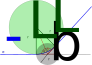
\includegraphics[width=0.5\columnwidth]{elecspec.png}
\caption{Visualisation of an electron deflected in a homogeneous circular magnetic field (grey) with radius $r_b$. The larger green circle indicates the Larmor radius, determining the electron trajectory (blue) from the point of entry into the field (A) to its exit point (C) resulting in a total deflection $\theta$.}
\end{figure}

Drawing the circular field region for the magnetic field and the electron entering the field, one can then graphically indicate its Larmor radius, equivalent to its expected motion for the region with the constant B-field. The angles in this constellation are determined using the trigonometric relation that the angles in a triangle have to add up to $\pi$:
\begin{equation}
2 \alpha + \theta = \pi,
\end{equation}
where $\theta$ is the deflection angle and $\alpha$ the angle indicated in the graphic (see figure).

Relating this to the angles to substitute $\alpha$:
\begin{equation}
\tan \alpha = \frac{r_L}{r_b},
\end{equation}
and then expressing this into parameters we can measure in experiment we reach
\begin{align}
\tan \frac{\theta}{2} &= \frac{r_b}{r_L},\nonumber\\
&= \frac{e B r_b}{p_\perp}.
\end{align}

In a typical LWFA experiment $p_\perp$ will be dominated by the component in the laser propagation axis, i.e. if the propagation axis were z, $|\mathbf{p_\perp}| \approx p_z$. 




The energy of the relativistic electrons are commonly measured by a spectrometer based on magnetic dispersion. In most wakefield setups at laser facilities or universities the relativistic charged particle beam is deflected by the field of a dipole magnet. In experiments located at conventional accelerator facilities the beam is often diverted and re-imaged using a series of dipole and quadrupole magnets. 
Finally, a scintillator screen, e.g. lanex, is positioned in the beam path and imaged by a camera. When all parameters, magnet strength, propagation distance, particle mass etc. are well-known, each position on the screen in the dispersion axis can be associated to an energy.
\vspace{\baselineskip}

\begin{figure}[h]
\includegraphics[scale=1.2]{magnet3.png}
\includegraphics[scale=0.12]{Espec_shotexemp.jpg}
\caption{Sketch of a typical spectrometer setup in a LWFA experiment (left). The relativistic electron beam enters the dipole magnet (grey) and is dispersed onto the lanex screen according to its energy. Higher energies are deflected less than lower energies. The image on the right is an example of a spectrum taken on an experiment. The high energies are on the top and the spectrum decreases downwards.}
\end{figure}

The correct assignment of the position on the screen to the correct electron energy is achieved by measuring the position of all components (lanex screen, magnet, TCC) and the magnet field strength accurately and then running a particle tracking code with these details.
Each pixel has a certain error bar on its associated energy as the divergence of the electron beam, an offset at source or shot-to-shot pointing fluctuations could lead to different positions at the same electron energy.
\vspace{\baselineskip}
\EliasComm{Present typical path from raw image and tracking to the end.}
\EliasComm{Make a new sketch.}
A second lanex screen or other spatial references (fiudicials) can help to identify and correct for pointing fluctuations or an overall pointing to achieve a more accurate determination of the energy.

The width of the electron trace in the non-dispersion direction can be used to determine the divergence of the beam and cross-checked with the spectrum of the betatron radiation.

In experiment, perfectly homogeneous fields are even in approximation rarely encountered, especially at the fringes of physical magnets the fields smoothly fall off to a zero background field. Hence, usually homogeneous fields are only used as approximation that can provide a rough estimate (see the analytic solution of the deflection angle in the theory section) and physical magnets are mapped using a Hall probe for instance before or after the experiment to achieve more accurate results. Even outside the magnet by-passing electrons can be influenced by fringe fields which can lead to deflection of electrons at low energies if the space is limited. This should be avoided or the fields need to be sufficiently shielded, e.g. by using mu-metal.


\subsubsection{Multiple screens and deconvolution}

In a magnetic spectrometer electrons are being dispersed in one axis and the spectrum can be deduced from the fan of electrons and the position at a detector screen. Whereas the spatial extent in the non-dispersion direction tells us the divergence of the beam in that axis as it is approximately unperturbed, the divergence of the beam in the dispersion direction is convolved with the magnetic dispersion. At the same time an overall pointing of the beam could lead to an overestimate or underestimate of the actual energy. In order to be able to correct for these factors several points of reference are required. The source position has to be known along with two more measurements. This could be two screens or a spatial feature (fiudicial) and one screen.
A simple symmetry assumption mainly allows adding an error bar to the maximum energy within a reasonable limit.

Two screen tracking: forwards or backwards method.
Run tracking with a variety of angles for identical energies. Check what energy estimate each screen gives at a distinct feature. See if there are any deviations, try the next angle and find the least square fit.
The other approach is backtracking but this is more complicated.

If one has a fiudicial no explicit features in the beam are required as the fiudicial will become that feature. However, the positions have to be measured to a high precision to be able to distinguish sensible pointing shifts.

Either methods can be used to deconvolve the spectrum and iteratively find the real energy spectrum udnerlying the measured distribution. More screens can increase the accuracy but the scattering of the beam passing through lanex becomes quite evident and distinct features blur out when drifting further because of this.

\EliasComm{Add an image for deconvolution.}

\subsection{Charge Measurement}

Absolute charge measurements are challenging in an EMP rich enviroment as intense laser-plasma interactions.
ICT Turbos have been attempted to be used in laser facilities but have only been successfully applied in facilities based on conventional facilities.

In other facilities image plates are being applied to find an absolute number for a certain range of shots which is then used to calibrate normal imaging systems giving a pixel count to charge conversion factor. The image plate is in our case attached to the back of the lanex scintillator screen such that for the respective shots the electron spectrum is being recorded on the lanex and on the imaging plate.
Image plate is light sensitive and is scanned after radiation/particle exposure at known conditions to extract the information.
The spatial resolution and dynamic range is superior to many cameras. The image from the camera and the imaging plate can be overlaid to find a suitable conversion factor. The scattering and damping of the imaging plate has to be considered and its heightened sensitivity which might result in additional background noise on the imaging plate due to its large dynamic range.

The downside of imaging plate technology is that it is not feasible as high repetition rate diagnostic. Any change of setup requires a new calibration.

\EliasComm{Add images from image plates from this run and how to overlap them.}

\section{X-ray and Gamma-ray Diagnostics}

Wakefield acceleration has not only demonstrated to be a feasible tool to accelerate electrons to a GeV scale, but has also been shown to be a useful source for X-rays of remarkable brightness, e.g. by the means of betatron radiation \cite{Rousse2004} or also as a tunable all-optical Compton-source \cite{TaPhuoc2012a}.

To decide whether a radiation source is suitable for certain applications, a thorough characterisation of its properties like flux, energy spectrum, source size, pulse duration and divergence is useful.
The following tools were used in the context of the author's work for this purpose.

\subsection{Gamma-ray Scintillator Profile}

When X-rays increase in energy and reach the gamma-ray regime (> 1 MeV), the direct detection of those photons with a camera on axis becomes less feasible as photons will decay into secondary particles and radiation that will shower the camera and reduce its lifetime.

Relying on indirect detection then becomes necessary. Using an array or a screen of scintillator. The shape of the profile is interesting as it allows deduction of the source. In this context it gives insight into the properties of the electrons (their divergence, propagation and so on). In case of ICS this also gives an idea of interaction intensity and polarisation of the beam.
To measure the divergence in both axes and as measurement of the intensity.

\subsection{Gamma-ray Converter Spectrometer}

At gamma-ray energies above 1 MeV one photon can generate a pair of electron-positron pairs when scattering on matter. The spectrum of the generated electrons and positrons are linked to the energy of the gamma photon. Based on this principle one method to measure the gamma spectrum is using a sheet of high-Z material to convert the gamma rays into matter and then measure the spectrum of these particles in a magnetic spectrometer (REF).

This works well for several MeV radiation but becomes less sensitive at higher energies (REF?) when the energy spectrum of the generated particles becomes less sensitive to the photon energy.
\EliasComm{Add an image.}

\subsection{Gamma-ray Scintillator Arrays}

One method to detect and characterise X-rays is using blocks or slaps of scintillating material extending in the propagation direction of the radiation or perpendicular to it, depending on what aspect of the radiation one is interested in. The response of the material, i.e. how photons or particles deposit energy and how the scintillator reacts, is then modelled using Monte-Carlo codes, e.g. GEANT4 \cite{Agostinelli2003} or MCNP \cite{Goorley2012}, and compared to the response measured. In general, the penetration depth and the energy deposited in the crystals are proportional to the energy of the radiation transmitted. To discriminate the spectrum even further, different materials can be overlaid as the response varies from material to material. This might be more complicated for very high energetic gamma rays as the cross section is almost identical for most materials at the MeV scale.

In contrast to other transmission studies the energy deposition and transmission is less linear but involves decays of photons into matter and those cascading back to photons. This means the signal will not follow a simple Beer's law but will require numerical solving and simulation via GEANT4 considering Bethe-Heitler processes etc.



\EliasComm{Deeper explanation of the setup and how the spectrum is being retrieved. Reference Keegan's paper.}
\EliasComm{Provide picture of the arrays.}

\subsubsection{Dual Axis Scintillator Array}

The new dual axis detector. Measure spectrum and divergence in two axes.


